\section{基于树与规则的分类}
\label{sec:classification-trees}

有些类别关系由局部条件决定：先检查一个特征，只有条件不满足时才需要查看另一个特征。例如图\ref{fig:classification-tree-partition}中的教学分类规则，在左半区域一律输出类1，在右半区域才由第二个坐标决定类别。一个全局线性得分不能精确表达整片区域中的这两段分界。分类树沿用第\ref{sec:classic-overview-tree-rules}节的条件分支，把输入逐步送入不同区域，再在叶节点输出类别或类别比例；路径中的先后测试使后续条件只在相应区域生效。

沿用训练集$D_n=\{(\bm{x}_i,y_i)\}_{i=1}^n$，其中输入有$d$个特征，$y_i\in\{1,\ldots,C\}$。本节允许特征是数值型或类别型，用$D\subseteq D_n$表示到达某个节点的训练样本。建树需要同时确定测试特征、阈值或取值分组，以及叶节点的输出，并非只估计一组预先固定的数值参数。常见做法是在当前节点选择一个能改善类别划分的测试，再递归处理各个子集；为避免把偶然差异也变成分支，还要限制生长或在生长后\term{剪枝}（pruning），即删除缺少预测收益的子树。

图~\ref{fig:classification-tree-partition}把同一个分类器分别画成区域和条件树。在$[0,1]^2$内，$x_1\leq0.5$的输入直接判为类1；其余输入继续检查$x_2$，不超过$0.55$时判为类2，否则判为类1。左图的水平分界只出现在右半区域，正对应右图中第二次测试只对第一个条件不成立的输入执行。这说明树中的路径不仅记录有哪些条件，也规定条件在哪个区域生效。

\begin{figure}[htbp]
  \centering
  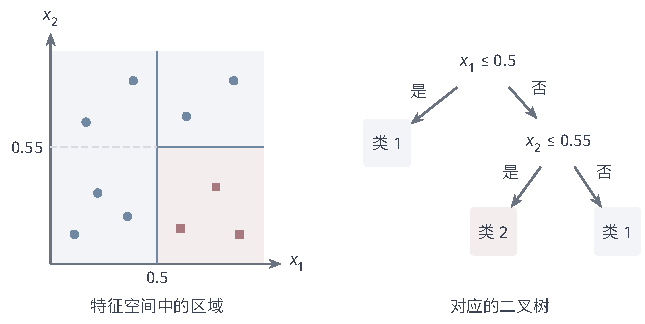
\includegraphics[width=109.241mm]{figures/04-classic-models/00-shared/tikz/classification-tree-partition/figure.pdf}
  \caption{二维分类的教学构造。左图为归一化特征空间$[0,1]^2$中的区域划分，圆点表示类1，方点表示类2；右图为产生同一划分的条件树。根节点检查$x_1\leq0.5$，仅在其“否”分支上继续检查$x_2\leq0.55$。点的位置与分裂阈值均为人为设定，不代表真实数据实验。}
  \label{fig:classification-tree-partition}
\end{figure}

不同树算法的主要差异落在三个问题上：怎样评价一次分裂，允许什么样的分支结构，怎样控制树的大小。ID3提供了信息增益驱动的基本构造，C4.5扩展其评分和数据处理方式；CART则采用统一的二叉划分与子树选择框架，形成了另一条决策树研究路线。

\subsection{ID3}
\label{sec:classification-id3}

要决定先检查哪个特征，需要比较“检查前还分不清多少类别”和“检查后还分不清多少类别”。ID3（Iterative Dichotomiser 3）据此选择特征，再在各分支上重复同一过程。Quinlan在1986年的论文中将ID3追溯到Hunt等人的概念学习系统（Concept Learning System, CLS）：CLS向前考察若干层候选树，按测量与误分类代价选择测试；ID3则改用信息驱动的局部评价。这一变化把建树中的“先测什么”落实为当前节点上可计算的信息增益比较，优化范围限定在当前节点的候选测试。本节采用以离散特征、信息增益和不作后剪枝为设定的基本ID3\scite{quinlan1986trees}。

\subsubsection{模型结构}
\label{sec:classification-id3-structure}

在节点样本集$D$上，记$p_c(D)$为类别$c$的样本比例。\term{熵}（entropy）用一个数概括类别分布的不确定性：节点只含一类时为零，各类越均匀，熵越大。采用以2为底的对数，
\begin{equation}
  H(D)=-\sum_{c=1}^{C}p_c(D)\log_2 p_c(D),
  \label{eq:classification-entropy}
\end{equation}
其中约定$0\log_2 0=0$。对第$j$个离散特征，令$V_j$为其可能取值集合，$D_{j,v}=\{(\bm{x}_i,y_i)\in D:x_{i,j}=v\}$。该特征的\term{信息增益}（information gain）是分裂前后熵的减少量：
\begin{equation}
  \operatorname{Gain}(D,j)
  =H(D)-\sum_{v\in V_j}\frac{|D_{j,v}|}{|D|}H(D_{j,v}).
  \label{eq:classification-information-gain}
\end{equation}
空子集对求和的贡献定义为零。这里必须按子集大小加权，否则只有一个样本的小分支会与包含大部分样本的分支同样重要。

ID3用选中的特征建立一个内部节点，每个取值对应一个分支。叶节点保存到达该处的类别计数，并通常输出多数类；类别计数相同时使用预先固定的平局规则。这样得到的是分段常值分类器：同一叶区域内的所有输入具有相同预测。叶节点也可报告类别频率，但少量样本上的频率不应被直接理解为可靠的概率估计。

信息增益把分裂选择变成了可计算的局部比较，却有\term{多值偏差}（multivalued attribute bias）：取值很多的特征更容易把训练样本分成纯净的小组。若每条记录的编号都不同，用编号分裂会使所有子节点熵为零，增益达到$H(D)$，但对一个新编号几乎没有帮助。

\subsubsection{参数学习}
\label{sec:classification-id3-learning}

从根节点的$D_n$出发，算法计算所有可用特征的信息增益，选择最大者，再分别对其子集递归建树。离散特征已经按取值完全展开后，同一路径上不必再次使用它。若当前样本全部同类，就生成该类叶节点；若可用特征耗尽而标签仍不一致，就输出当前多数类。对训练时未出现的分支，可以保留以父节点多数类为输出的回退叶节点，使预测规则对新输入仍有定义。

每次选择只依据当前节点，因而这是\term{贪心搜索}（greedy search）：接受眼前收益最大的分裂，不回头枚举所有可能的整棵树。基本ID3不在建树后再作剪枝；限制最大深度、最小叶样本数或最小增益，属于另外加入的生长控制。尤其是“增益为零就停止”也会改变基本搜索行为：在异或关系中，单个特征的增益可能为零，而连续两次测试可以完全分开类别。停止规则既能减少无效分裂，也可能阻止发现特征交互。

\subsubsection{理论分析}

\paragraph{表达能力}
对有限取值特征，若允许一条路径检查全部$d$个特征、保留至多$\prod_j|V_j|$个叶，就能为每个取值组合单独指定类别。因此任意只依赖这些字段的确定性类别映射都在这个树类中；有标签噪声时，完整组合上的类别分布也可由相应叶的概率向量表示。逐层组合坐标条件使树能够表示高阶交互。例如四点异或只需先检查$x_1$、再在两个分支分别检查$x_2$，深度为2、叶数为4；一层树却只能按一个坐标分组，在等概率四点上至少有一半标签无法吻合。

一旦限制深度或合并叶，尚未区分的取值组合就必须共用预测。这个限制不能靠增加同类样本消除。同一份特征记录若对应不同标签，树也无法逐条区分，只能用类别分布或多数类概括该处的随机性。



\paragraph{收敛性}
离散特征在同一路径最多使用一次，因此树深度至多为$d$，递归必然停止。每层所有非空节点合计处理至多$n$条记录；按每个节点扫描剩余字段的直接实现，建树成本至多为$O(nd^2)$，不计显式列出未观测空分支的成本。有限树类中的最小训练错误一定存在，但逐节点最大化信息增益并不求解这个全局问题，不能把递归结束理解为找到了训练错误最小的树。

\paragraph{泛化性}
\begin{theorem}[ID3在有限离散输入下的期望分类风险界]
固定各字段的有限取值集合，令$V=\prod_j|V_j|$。完整输入组合上的确定性分类器至多有$C^V$个；ID3返回的树，无论如何选择分裂，都属于这个固定集合。由式\eqref{eq:regression-finite-class-deviation}，对$n$个独立同分布的训练样本，以至少$1-\delta$的概率，
\[
 R_{01}(\hat h)\leq\widehat R_{01}(\hat h)
       +\sqrt{\frac{V\log C+\log(2/\delta)}{2n}}.
\]
\end{theorem}

这个界直接覆盖由训练数据选出的树，却可能因输入组合太多而没有实用精度。限制树的规模可以缩小候选数；未预先限定的新类别取值或连续阈值不满足这里的有限输入假设。

\subsubsection{优化泛化能力}

若关注的不只是类别变纯，还包括分裂是否有足够的统计证据，可以采用Kass于1980年提出的\term{卡方自动交互检测}（chi-square automatic interaction detection, CHAID）。它对类别特征的取值与标签建立列联表，先合并类别分布差异不显著的取值，再比较各特征与响应的关联，按经过多重比较调整的检验结果选择分裂；证据不足时停止。剩下的取值组形成多路分支，适合把分群结果读作交叉分类，但连续变量通常需要先分组，分组方式会影响结果。检验显著性针对相应的关联原假设，树的预测误差还需另行评价\scite{kass1980chaid}。

\subsubsection{小结}
\label{sec:classification-id3-summary}

ID3把离散字段逐层组织为类别区域，用当前节点的信息增益决定下一次测试。取值很多的字段容易获得较高增益，训练噪声也可能被写成细小分支。关联检验提供了另一种控制生长的依据，C4.5则继续调整评分和数据处理；应区分测试能表达什么与搜索为何选择它。

\subsection{C4.5}
\label{sec:classification-c45}

ID3的基本构造已经能从离散特征递归建树，但前面用记录编号的例子说明，信息增益会偏爱把训练样本切得很细的特征。实际记录还常有连续测量值和缺失字段：不能为每个长度值都建立一条新分支，也不能遇到未知值就让预测失去定义。让树处理这些数据，需要同时调整测试评分、阈值选择与缺失记录的传递方式。

Quinlan在1993年的专著中给出了C4.5的完整程序体系。它沿用ID3的递归构造，用增益率抑制部分多值偏差，通过阈值测试处理连续变量，并以分数权重传递缺失记录；树长成以后，再用错误估计剪枝和规则提取控制结构。以下分别说明这些机制如何工作\scite{quinlan1993c45}。

\subsubsection{模型结构}
\label{sec:classification-c45-structure}

多值特征容易得到大增益，是因为它本身就把数据切得很细。C4.5用\term{信息增益率}（gain ratio）比较“类别信息的增加”与“产生这些分支所需的划分信息”。设测试$a$把$D$分成$D_1,\ldots,D_b$，令$q_v=|D_v|/|D|$，则
\begin{align}
  \operatorname{SplitInfo}(D,a)
  &=-\sum_{v=1}^{b}q_v\log_2 q_v,
  \label{eq:classification-split-information}\\
  \operatorname{GainRatio}(D,a)
  &=\frac{\operatorname{Gain}(D,a)}
  {\operatorname{SplitInfo}(D,a)}.
  \label{eq:classification-gain-ratio}
\end{align}
这里的信息增益仍按式\eqref{eq:classification-information-gain}计算，只把按特征取值划分替换为测试$a$的各个结果。分母为零意味着没有真正划分，不能参与比值比较。

小分母会改变增益率的排序：只分离少量样本的测试具有较小的划分信息，微小信息增益也可能得到较大比值。C4.5先计算候选的平均信息增益，再在增益不低于平均值的测试中比较增益率。这个启发式筛选限制依靠小分母取胜的候选，实际预测价值仍由独立验证评价。

\subsubsection{参数学习}
\label{sec:classification-c45-learning}

离散特征可以按取值作多路分裂；连续特征则使用$x_j\leq t$与$x_j>t$的二路测试。候选阈值来自排序后相邻不同取值之间，且分裂后必须满足最小子节点样本量等限制。连续特征在某次分裂后仍可在后代节点使用，因为同一数值轴上可能需要多个阈值。

C4.5各版本对阈值的评价略有区别。较早版本按增益率选择阈值；Quinlan在1996年的修订中先按信息增益选择连续特征的阈值，再扣除搜索阈值所需的描述长度代价，参与特征之间的增益筛选和增益率比较。若有$q$个候选切分位置，这项逐样本惩罚形如$\log_2 q/|D|$，用来抵消“可试阈值更多”带来的选择优势。算法~\ref{alg:classification-c45}突出这些版本共有的建树骨架，把阈值评价留在候选测试生成步骤中\scite{quinlan1996continuous}。

\begin{algorithm}[C4.5的递归生长与后剪枝]
  \label{alg:classification-c45}
  \begin{algorithmic}[1]
    \Require 节点样本$D$，可用特征集合$F$，停止及剪枝设置
    \Ensure 剪枝后的分类树
    \Function{Grow}{$D,F$}
      \If{$D$全部同类，或样本量不足，或$F$为空}
        \State \Return 以$D$中多数类为输出的叶节点
      \EndIf
      \State 生成各特征的有效测试，连续特征同时选择阈值
      \State 计算各测试的增益；缺失值按正文约定处理
      \If{没有有效测试，或最大增益不为正}
        \State \Return 以$D$中多数类为输出的叶节点
      \EndIf
      \State 求候选测试的平均增益$\bar g$
      \State 保留增益不低于$\bar g$且划分信息为正的测试
      \State 选择其中增益率最大的测试$a$，建立节点$T$
      \For{测试$a$的每个结果$v$}
        \State 得到相应的子集$D_v$及子问题的特征集合$F_v$
        \If{$D_v$为空}
          \State 将$D$的多数类叶节点接到分支$v$
        \Else
          \State 将$\Call{Grow}{D_v,F_v}$接到分支$v$
        \EndIf
      \EndFor
      \State \Return $T$
    \EndFunction
    \State $T\gets\Call{Grow}{D,F}$
    \State 自底向上比较子树与简化方案的悲观错误估计
    \State \Return 剪枝后的$T$
  \end{algorithmic}
\end{algorithm}

缺失值需要在评分和路由中保留不确定性。设测试$a$的已知样本总权重占当前节点的比例为$q_{\mathrm{known}}$，C4.5在已知样本上估计熵下降，再乘$q_{\mathrm{known}}$降低该测试的收益；划分信息也计入未知部分。选择测试后，缺失记录按已知样本进入各分支的比例作分数权重分配，后续熵、类别计数和多数类都使用这些权重。预测遇到缺失值时，也按分支权重综合子树输出。

树生长完成后，C4.5采用\term{悲观错误剪枝}（pessimistic error pruning）：训练误差倾向于低估新样本错误，因而以二项错误计数的上置信估计作修正，比较保留子树与折叠成多数类叶节点的估计错误数。若简化方案不更差，就可以删除该子树；完整实现还可考察用某个子树提升替代当前分支。置信设置控制剪枝强度，这一自适应建树后的估计用于启发式模型选择，整树的样本外错误仍通过验证或测试数据评价。

树也可以转成规则：每条根到叶路径的测试构成规则前件，叶类别作为后件，再尝试删除不必要条件并筛选规则。未经简化的路径规则继承树的区域划分；条件删除以后可能产生重叠，因此规则系统还必须规定冲突处理和默认预测。这种转换并非只把树的文字抄成一份无序清单。

\subsubsection{理论分析}

\paragraph{表达能力}
连续特征的单坐标阈值把每个叶区域限制为坐标区间的交，也就是轴对齐的矩形或更高维的长方体。几个这样的区域可以精确表达前面的分段教学规则，却不能用有限条轴对齐边界精确重现整条斜线。表示限制在于分区方向，增益率只改变选择哪次分裂。

这个差距可以随着树的规模减小。例如，设输入在$[0,1]^2$上均匀分布，真实类别由$x_2>x_1$决定。把$x_1$轴等分为$m$个宽度$1/m$的区间，在每个区间内以其中点作为$x_2$阈值，至多$2m$个叶就能形成阶梯边界。每个竖条内与目标不一致的面积为$1/(4m^2)$，合计为$1/(4m)$。因此，至多$2m$叶的候选族中存在一个标签不一致比例为$1/(4m)$的表示。缺失字段的输入则没有提供该坐标的真实值；若两个对象的已观测字段相同，仅依赖这些字段的候选无法区分它们。



\paragraph{收敛性}
对完整输入，合法分裂将节点中的样本分为至少两个非空子集，沿任一路径的样本数严格减少，故至多$n$个非空叶后生长结束。缺失记录按权重分流时，不能继续用这条整数计数证明；实现需明确最小有效样本量，并可用预定最大深度保证有限终止。剪枝对有限树作有限次替换，同样会结束。增益率与局部错误估计都不是整棵树训练目标的精确求解器，因此没有由这些步骤自动推出的全局最优收敛率。

\paragraph{泛化性}
\begin{theorem}[C4.5冻结候选树在独立验证下的期望风险界]
连续阈值由训练数据确定，缺失输入还可能混合多个分支，因而不能只数最终树上出现的阈值来控制训练偏差。可以先用生长数据生成$J$棵完整预测规则固定的候选树，再在独立的$m$个同分布验证样本上选择错误率最小的$\hat h$。条件于这些候选树，零一损失的Hoeffding界与并集界给出，以至少$1-\delta$的概率，
\[
 R_{01}(\hat h)\leq\min_{1\leq j\leq J}R_{01}(h_j)
            +2\sqrt{\frac{\log(2J/\delta)}{2m}}.
\]
\end{theorem}

前一项保留候选树本身的质量，后一项控制验证选择的误差。该结论适用于这一独立验证协议，不能替换为C4.5内部的悲观错误估计；反复读取同一验证集来生成新树也不满足冻结候选的条件。

\subsubsection{优化泛化能力}

来自不同抽样来源的记录，未必应有相同训练权重。C4.5之后的C5.0加入了样本权重、误分类代价和特征筛选等功能\scite{rulequest2017c50}。样本权重调节不同记录在拟合中的贡献，让树与规则的选择更接近所关注的数据分布。权重需要有相应的抽样或评价依据；任意放大某些记录的贡献并不保证降低总体风险。

\subsubsection{优化计算能力}

数据规模增加时，树或规则生成过程的时间与内存也会限制使用。C5.0在C4.5之后继续改进这些实现；RuleQuest提供商业版本和GPL源码版本，其公开实验报告了特定数据与硬件条件下的速度及内存改进\scite{rulequest2017c50}。比较时应固定数据、硬件和输出形式，因为生成树与生成规则集的开销可以不同。实现上的节省与误分类代价设置处理的是不同问题，需要分别记录资源消耗和分类错误。

\subsubsection{支持误分类代价不同的场景}

邮件过滤中，误拦一封正常邮件与漏放一封垃圾邮件可能具有不同代价。误分类代价把这种差异写入损失，使树与规则按所关心的错误代价评分和选择。这里扩展的是评价目标，预测仍使用相应的树或规则表示。

\subsubsection{小结}
\label{sec:classification-c45-summary}

C4.5在ID3式递归划分中补充分裂评分、连续阈值、缺失字段传递与后剪枝，并可把路径转成规则。它处理的困难不只是分裂后类别是否更纯，还包括记录怎样经过分支，以及长成的树应保留多少细节。

C5.0继续改善树与规则生成，并使训练能够考虑样本权重和误判代价。实现效率与实际决策中的错误成本因而进入选择，但仍应检查所用字段是否有意义、缺失值如何影响预测，以及最终条件能否被审阅。

\subsection{CART}
\label{sec:classification-cart}

另一种组织树的方法是把每次测试都限定成二选一，再统一研究大树中应保留哪些子树。\term{分类与回归树}（classification and regression trees, CART）采用这一框架；Breiman、Friedman、Olshen与Stone在1984年的专著中将树的构造、最优剪枝与统计性质放在同一体系中讨论。其中，代价复杂度剪枝把“怎样长出一棵大树”与“最终保留多大的子树”分开：生长阶段比较局部分裂，剪枝阶段形成候选子树序列，再用验证选择规模。因此，CART与ID3的区别不只是换一个不纯度指标，还涉及分支结构与整树选择。这里关注分类树；第\ref{sec:regression-cart}节的回归CART复用递归二分与代价复杂度剪枝，但按响应损失选择分裂并在叶内输出数值，本节则按类别不纯度或误分类代价分裂并输出类别标签或类别比例\scite{breiman1984cart}。

\subsubsection{模型结构}
\label{sec:classification-cart-structure}

CART分类树通常用\term{基尼不纯度}（Gini impurity）评价节点中类别的混杂程度：
\begin{equation}
  G(D)=1-\sum_{c=1}^{C}p_c(D)^2.
  \label{eq:classification-gini}
\end{equation}
它也等于从节点经验类别分布独立抽取两个标签时，两者不同的概率。对于产生左右子集$D_{\mathrm{L}}$和$D_{\mathrm{R}}$的测试$a$，比较
\begin{equation}
  \Delta G(D,a)=G(D)
  -\sum_{v\in\{\mathrm{L},\mathrm{R}\}}
  \frac{|D_v|}{|D|}G(D_v).
  \label{eq:classification-gini-decrease}
\end{equation}
基尼与熵都鼓励子节点变纯，但并不总给出相同的排序。基尼计算省去对数运算，整棵树的训练成本还包含阈值搜索与数据访问。

对连续特征，二分测试仍是阈值比较；对类别特征，测试可写成$x_j\in S$与$x_j\notin S$，其中$S$是部分取值组成的集合。寻找这个集合本身也是搜索问题，候选分组数随取值数增加，搜索成本需要计入建树预算。统一的二叉结构便于遍历和剪枝，但可能用多层测试表达一棵多路树的一次分裂。

\subsubsection{参数学习}
\label{sec:classification-cart-learning}

生长阶段反复选择基尼下降最大的有效二分测试，直到满足生长限制，得到一棵较大的树$T_0$。随后进行\term{代价复杂度剪枝}（cost-complexity pruning）：不再逐个比较局部增益，而是在$T_0$的候选子树中平衡拟合误差和叶节点数。令$L(T)$为树$T$的叶节点集合，$\hat c_\ell$为叶$\ell$的预测类别，定义
\begin{align}
  \widehat R(T)
  &=\frac{1}{n}\sum_{\ell\in L(T)}
    \sum_{(\bm{x}_i,y_i)\in D_\ell}
    \mathbb{1}\{y_i\neq\hat c_\ell\},
  \label{eq:classification-cart-empirical-risk}\\
  J_\alpha(T)&=\widehat R(T)+\alpha|L(T)|,
  \qquad \alpha\geq0.
  \label{eq:classification-cart-cost-complexity}
\end{align}
这里$\widehat R(T)$采用全训练集上的误分类比例，使不同子树的误差具有共同尺度。有些软件把叶不纯度的加权和作为剪枝代价；使用其参数时需要核对具体定义，再按该尺度解释$\alpha$。

剪枝路径可以由\term{最弱环节剪枝}（weakest-link pruning）生成。设内部节点$t$以下的子树为$T_t$，把它折叠成一个叶节点后，该区域对全训练集误差的贡献为$\widehat R(t)$；保留时贡献为$\widehat R(T_t)$。两种方案的代价相等时，
\begin{equation}
  \alpha_t=
  \frac{\widehat R(t)-\widehat R(T_t)}
       {|L(T_t)|-1}.
  \label{eq:classification-weakest-link}
\end{equation}
分子是折叠后增加的训练错误，分母是删去的叶数，因而$\alpha_t$衡量“每少保留一个叶节点要付出多少误差”。剪去最小$\alpha_t$对应的分支，再重新计算，就得到从大树到根叶节点的嵌套序列。若某些分支增加叶数却不降低误分类率，可先在$\alpha=0$时合并；临界值处可能有多个最优子树，按一致的最小子树约定处理平局。

对每个$\alpha$，上述序列包含相应的最优剪枝子树，最优性范围限定为给定$T_0$的剪枝子树。实际需要用验证集或交叉验证选择$\alpha$；交叉验证时，在各训练折内独立生长和剪枝，再评价对应验证折。

预测还要规定主测试字段缺失时如何分支。CART的\term{替代分裂}（surrogate split）寻找其他特征测试，按它们复现主分裂结果的程度选择替代；类别权重和误分类代价也可以改变生长与叶预测。具体实现采用哪些机制，需要与数据处理方式一同检查。

\subsubsection{理论分析}
\label{sec:classification-cart-theory}

\paragraph{表达能力}
CART与完整输入上的C4.5共享单坐标阈值的矩形分区能力，前面$2m$个叶、错误率$1/(4m)$的斜线逼近也可由二叉树实现。有限离散输入上的任意取值映射同样可以逐次二分展开，但叶数必须足以区分所需组合。二叉与多路的区别主要影响树深和条件复用，并不使基尼评分获得一种新的边界形状。

测试全集还会留下独立于叶数的限制。若两个输入对全部允许测试都给出相同结果，无论树怎样增长，它们都会走到同一叶，必须得到相同类别。测试集合固定时，增加叶数只能细化已允许的测试组合；目标所需的阈值或特征不在测试集合中时，逼近差距仍然存在。



\paragraph{收敛性}
在无缺失、每次产生两个非空子节点的设定下，生长至多产生$n$个非空叶。成本复杂度剪枝从这棵有限大树出发，每次减少内部节点，剪枝路径也有限。对固定叶数上限和有限测试集，全局最优树存在；但贪心生长不保证找到它。剪枝的最优性只针对给定大树的子树，不能扩展为所有可构造树的最优性。

\paragraph{泛化性}
节点类别变纯，是当前训练子集上的变化；要控制整棵树在新样本上的错误，还要把选测试、选结构和选叶标签造成的选择范围计入。先考虑一个明确受限的版本：输入没有缺失，抽样前给定有限测试集合，并限制最多保留多少个叶节点。
\begin{theorem}[CART在固定测试集与叶数约束下的期望分类风险界]
  \label{thm:classification-tree-risk}
  设训练样本独立同分布，类别数为$C\geq2$。抽样前固定$Q\geq1$个二值测试和叶数上限$L\geq1$；候选类$\mathcal T_{Q,L}$包含用这些测试构造、至多$L$个叶、各叶输出一个类别的所有二叉树。令
  \[
    u_{\mathrm T}=
      \sqrt{\frac{\log(2L/\delta)
        +(L-1)\log(4Q)+L\log C}{2n}},
       \qquad0<\delta<1.
  \]
  CART学习器通过生长与剪枝返回$\hat T\in\mathcal T_{Q,L}$。至少以$1-\delta$的概率，
  \[
    R_{01}(\hat T)
      \leq\widehat R(\hat T)+u_{\mathrm T}.
  \]
  在同一事件上，若
  $e_{\mathrm{opt}}=\widehat R(\hat T)
      -\min_{T\in\mathcal T_{Q,L}}\widehat R(T)$，则
  \[
    R_{01}(\hat T)-R^\ast
      \leq\inf_{T\in\mathcal T_{Q,L}}R_{01}(T)-R^\ast
            +2u_{\mathrm T}+e_{\mathrm{opt}}.
  \]
\end{theorem}
\begin{proof}
  有$\ell$个叶的有序满二叉树形状数为第$\ell-1$个Catalan数，至多$4^{\ell-1}$。每个内部节点有$Q$种测试，每个叶有$C$种输出，所以
  \[
    |\mathcal T_{Q,L}|
       \leq\sum_{\ell=1}^L4^{\ell-1}Q^{\ell-1}C^\ell
       \leq L(4Q)^{L-1}C^L.
  \]
  零一损失位于$[0,1]$，对这个预定有限类应用式\eqref{eq:regression-finite-class-deviation}的一致偏差界，便得$u_{\mathrm T}$。该事件同时覆盖全部候选树，因此也覆盖依训练数据选出的$\hat T$。用它先比较$R_{01}(\hat T)$与$\widehat R(\hat T)$，再加上$e_{\mathrm{opt}}$并与任意候选树比较，最后把候选树的经验风险换回期望风险，即得第二个结论。
\end{proof}

这里不要求CART找到所有树中的经验最优解；贪心生长和给定大树内的最优剪枝，未必使$e_{\mathrm{opt}}$为零。第一个界对任意返回的受限树成立，第二个界则保留它与候选类经验最优者的搜索差距。叶数增多可能减小逼近差距，却同时增大抽样误差项。

在完整的有限类别输入上，ID3与C4.5的多路测试也可以展开为若干二值测试；若测试全集和叶数上限预先固定，展开后的树满足同一个结论。通常实现从训练数值中挑选连续阈值，或对缺失输入混合分支预测，这些情形没有自动满足上述有限类假设。尤其不能在建树之后，把实际考察过的测试数当作预定的$Q$。若对独立验证集上的一条预先生成剪枝路径选择子树，可以条件于生长数据，再按候选子树数控制验证选择；其风险依据来自验证抽样，而不是节点不纯度本身。

\subsubsection{优化表达能力}

常数叶用一个概率向量概括区域中的全部输入；若同一区域内的概率仍随特征变化，可以保留树的划分，改变叶节点如何预测。\term{逻辑模型树}（logistic model tree, LMT）在每个叶区域内使用Logistic回归，即用特征的线性得分表示类别对数几率，再转成类别概率。这样，树负责不同区域之间的结构变化，叶模型负责区域内部随特征变化的概率。Landwehr、Hall与Frank的2005年期刊论文基于其2003年会议工作，结合C4.5分裂与CART剪枝形成树结构，并通过LogitBoost逐步拟合逻辑模型。在后代节点继续细化祖先模型，可以避免每个小叶都从零估计全部系数\scite{landwehr2005lmt}。

例如在二分类叶区域$\ell$内，LMT可输出
\begin{equation}
  \hat p_\ell(y=1\mid\bm{x})
  =\frac{1}{1+\exp[-(\bm{w}_\ell^\top\bm{x}+b_\ell)]},
  \label{eq:classification-lmt-leaf}
\end{equation}
其中$\bm{w}_\ell\in\mathbb{R}^d$和$b_\ell\in\mathbb{R}$是叶模型的系数。概率在单个叶区域内部平滑变化，但跨越不同叶的边界时仍可能跳变，也不自动具有良好的校准性质。模型拟合、迭代次数选择和树剪枝共同增加训练成本，解释时也要同时阅读路径条件与叶模型系数。
LMT能精确表达“各叶区域内对数几率分别为仿射函数”的后验，只要树能够形成这些区域。普通常值叶只能用一个概率概括叶内全部输入；LMT可以保留其中的线性变化，却仍不能在具有非零长度的连续输入区间内精确表达$x^2$这样的对数几率。进一步划分区域能够改善逼近，不能免除叶数与样本覆盖的限制。

\subsubsection{优化泛化能力}

信息增益和基尼下降还面临另一种偏差：候选切分越多，越容易偶然找到一个高分切分。\term{条件推断树}（conditional inference tree, CTree）把“选哪个特征”与“在该特征上怎样切分”分开。Hothorn、Hornik与Zeileis在2006年的框架中用条件置换分布评价特征与响应的关联：先检验当前节点中所有特征均与响应无关联的全局原假设；不能拒绝时停止，否则选择检验证据最强的特征，再为它寻找二分位置。通过同一检验尺度和多重检验控制，可以缓解不同取值数目带来的选择偏差\scite{hothorn2006ctree}。

CTree的置换检验依赖原假设下的可交换性，渐近近似的精度也受样本量影响。检验控制当前节点是否继续分裂，全树的预测质量仍应在独立数据上评价。

检验驱动的生长也有搜索边界：四点异或在两层树中可被精确表示，但根节点的每个单坐标都与标签独立，单变量检验可能阻止继续分裂。检验决定当前节点是否继续搜索，并不改变候选树本来能够表示的关系。

\subsubsection{小结}
\label{sec:classification-cart-summary}

把叶节点多数类换成数值均值，把分类不纯度换成平方误差，就得到平方损失下的回归树构造；不需要另换一种树的表示。多个树怎样组合，见第\ref{chap:ensemble-learning}章。

CART把二叉分裂的局部选择与整树规模的验证选择分开。条件推断树采用另一种分裂依据，先比较特征与类别的关联，再确定切分位置；这种选择针对候选切分数影响评分的问题。

若常数叶遗漏区域内部的概率变化，逻辑模型树可以在叶内使用特征得分，并结合C4.5分裂与CART剪枝组织区域。代价是还要拟合和选择叶模型，解释时同时阅读路径与系数。分裂选择、树的规模和叶内预测各处理不同困难，类别不平衡、缺失字段与误判代价也须在对应机制中处理。
